\documentclass[11pt,a4paper]{article}
\usepackage[margin=18mm]{geometry}
\usepackage{amsmath}
\usepackage{booktabs}
\usepackage{float}
\usepackage{graphicx}
\usepackage{subcaption}
\usepackage{xcolor}
\graphicspath{{figures/}}
\setlength{\parindent}{0pt}
\setlength{\parskip}{4pt}
\renewcommand{\arraystretch}{1.12}

\begin{document}
\begin{center}
{\Large\bfseries ASSIGNMENT 5: MAXIMUM LIKELIHOOD ESTIMATION}\\[3pt]
{\small 26AI5707 - Pattern Recognition and Machine Learning}\\[7pt]
{\small KARTHIKEYAN M (26120004) \quad MIRTHULA R (261200121)}\\[2pt]
{\small Shiv Nadar University, Chennai \quad October 2026}
\end{center}
\vspace{2mm}\hrule\vspace{5mm}

\section*{Part 1: Synthetic data}
\begin{center}
\begin{tabular}{ll}
\toprule
Classes & Three 2-D Gaussian classes \\
Means & $(0,0)$, $(4,0)$, $(2,4)$ \\
Samples & 10,000 per class \\
Train/test & 8,000 / 2,000 per class \\
Covariances & Isotropic, diagonal, full; shared and class-specific \\
\bottomrule
\end{tabular}
\end{center}
\vspace{6mm}
\subsection*{Estimator and decision rule}
\[
\hat{\boldsymbol\mu}_k=\frac{1}{N_k}\sum_i\mathbf{x}_{ki},\qquad
\hat{\boldsymbol\Sigma}_k=\frac{1}{N_k}\sum_i
(\mathbf{x}_{ki}-\hat{\boldsymbol\mu}_k)
(\mathbf{x}_{ki}-\hat{\boldsymbol\mu}_k)^{\mathsf T}.
\]
\[
g_k(\mathbf{x})=-\tfrac12(\mathbf{x}-\hat{\boldsymbol\mu}_k)^{\mathsf T}
\hat{\boldsymbol\Sigma}_k^{-1}(\mathbf{x}-\hat{\boldsymbol\mu}_k)
-\tfrac12\log|\hat{\boldsymbol\Sigma}_k|.
\]
Shared estimates pool class residuals. Diagonal and isotropic estimates retain their required structure.
The three class priors are equal, so the prior term does not change the predicted class.

\vspace{6mm}
\subsection*{Test accuracy}
\begin{center}
\begin{tabular}{lcc}
\toprule
Covariance & Shared (\%) & Different (\%) \\
\midrule
Isotropic & 97.20 & 89.05 \\
Diagonal & 82.73 & 87.37 \\
Full & 94.45 & 87.53 \\
\bottomrule
\end{tabular}
\end{center}
\vspace{8mm}
{\small\color{gray}Part 2: assigned real-data file not yet available.}
\newpage
\section*{Isotropic covariance}
\textit{Covariance entries below show $\sigma^2$.}
\begin{figure}[H]
\centering
\begin{subfigure}[t]{0.48\textwidth}
\centering
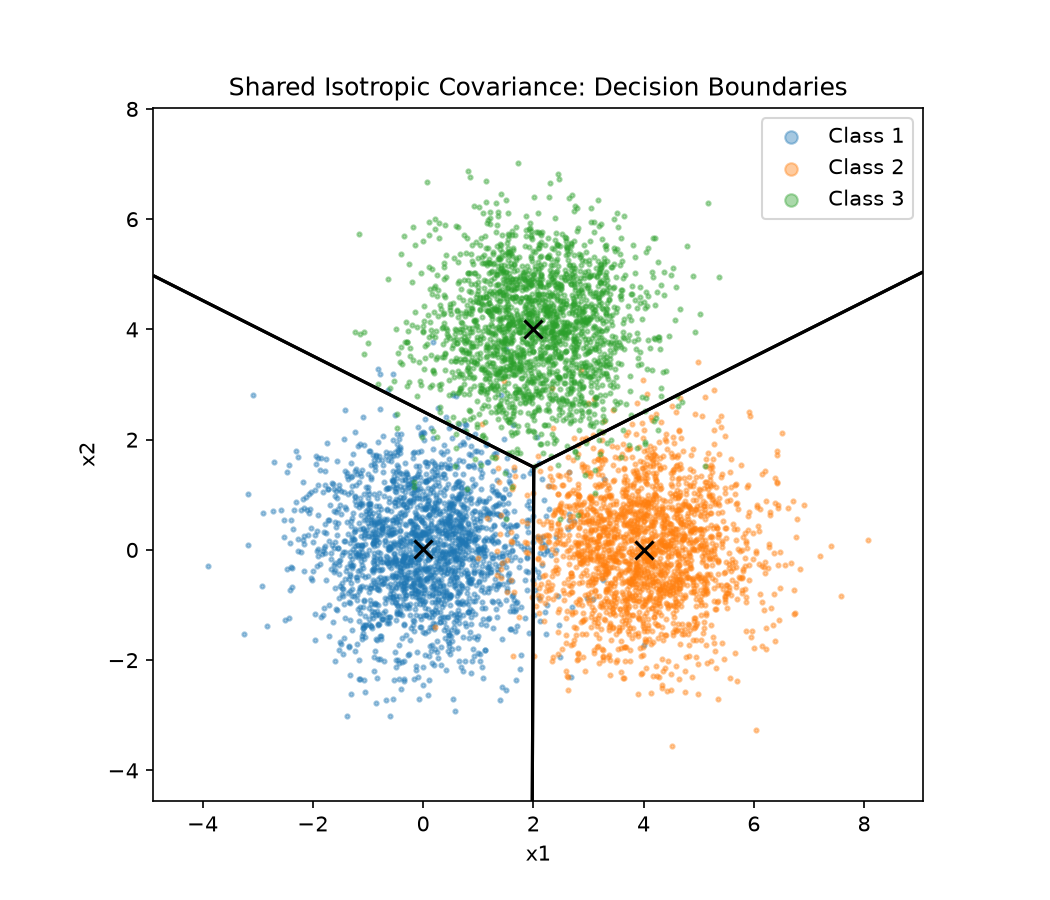
\includegraphics[width=\linewidth]{shared_isotropic_boundary.png}
\caption{Shared covariance}
\end{subfigure}
\hfill
\begin{subfigure}[t]{0.48\textwidth}
\centering
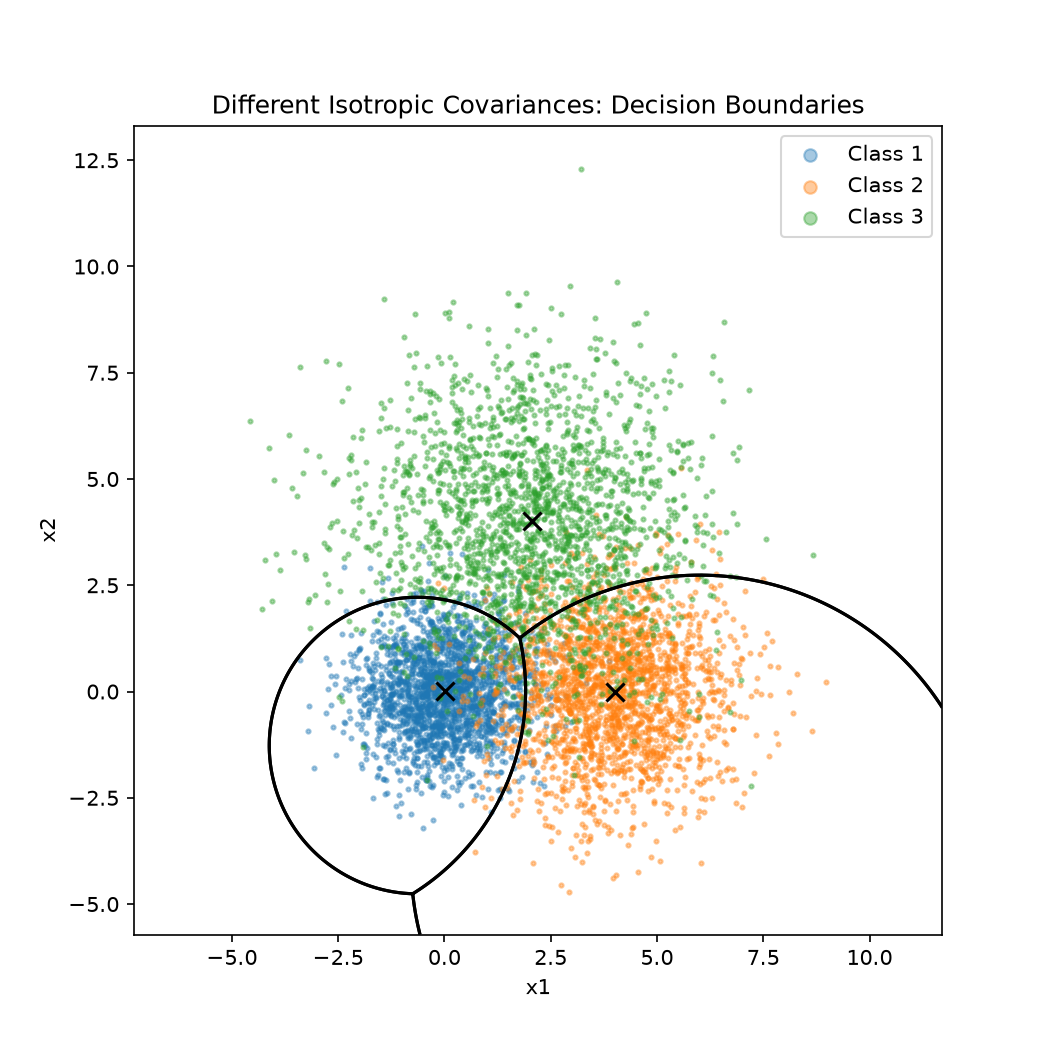
\includegraphics[width=\linewidth]{different_isotropic_boundary.png}
\caption{Different covariance}
\end{subfigure}
\caption{Test points and decision boundaries for isotropic covariance.}
\end{figure}
\vspace{7mm}
\begin{minipage}[t]{0.48\textwidth}
\small
\textbf{Shared: 97.20\% accuracy}\\[3pt]
\textbf{Estimated means}\\[-2pt]
\begin{tabular}{ccc}
\toprule
Class & $\hat\mu_1$ & $\hat\mu_2$ \\
\midrule
1 & -0.01 & 0.02 \\
2 & 4.01 & -0.00 \\
3 & 2.00 & 4.00 \\
\bottomrule
\end{tabular}\\[5pt]
\textbf{Covariance: generating / estimated}\\[-2pt]
\begin{tabular}{cll}
\toprule
Class & Generating & Estimated \\
\midrule
1 & 1.00 & 1.01 \\
2 & 1.00 & 1.01 \\
3 & 1.00 & 1.01 \\
\bottomrule
\end{tabular}\\[5pt]
\textbf{Confusion matrix} (rows: true; columns: predicted)\\[-2pt]
\begin{tabular}{c|ccc}
 & 1 & 2 & 3 \\
\hline
1 & 1934 & 45 & 21 \\
2 & 35 & 1944 & 21 \\
3 & 18 & 28 & 1954 \\
\end{tabular}
\end{minipage}
\hfill
\begin{minipage}[t]{0.48\textwidth}
\small
\textbf{Different: 89.05\% accuracy}\\[3pt]
\textbf{Estimated means}\\[-2pt]
\begin{tabular}{ccc}
\toprule
Class & $\hat\mu_1$ & $\hat\mu_2$ \\
\midrule
1 & 0.02 & 0.01 \\
2 & 4.02 & -0.01 \\
3 & 2.05 & 4.01 \\
\bottomrule
\end{tabular}\\[5pt]
\textbf{Covariance: generating / estimated}\\[-2pt]
\begin{tabular}{cll}
\toprule
Class & Generating & Estimated \\
\midrule
1 & 1.00 & 0.98 \\
2 & 2.00 & 2.04 \\
3 & 4.00 & 4.07 \\
\bottomrule
\end{tabular}\\[5pt]
\textbf{Confusion matrix} (rows: true; columns: predicted)\\[-2pt]
\begin{tabular}{c|ccc}
 & 1 & 2 & 3 \\
\hline
1 & 1872 & 75 & 53 \\
2 & 106 & 1776 & 118 \\
3 & 118 & 187 & 1695 \\
\end{tabular}
\end{minipage}
% Add observations in the student's own words.
\newpage
\section*{Diagonal covariance}
\textit{Covariance entries below show $(\Sigma_{11},\Sigma_{22})$.}
\begin{figure}[H]
\centering
\begin{subfigure}[t]{0.48\textwidth}
\centering
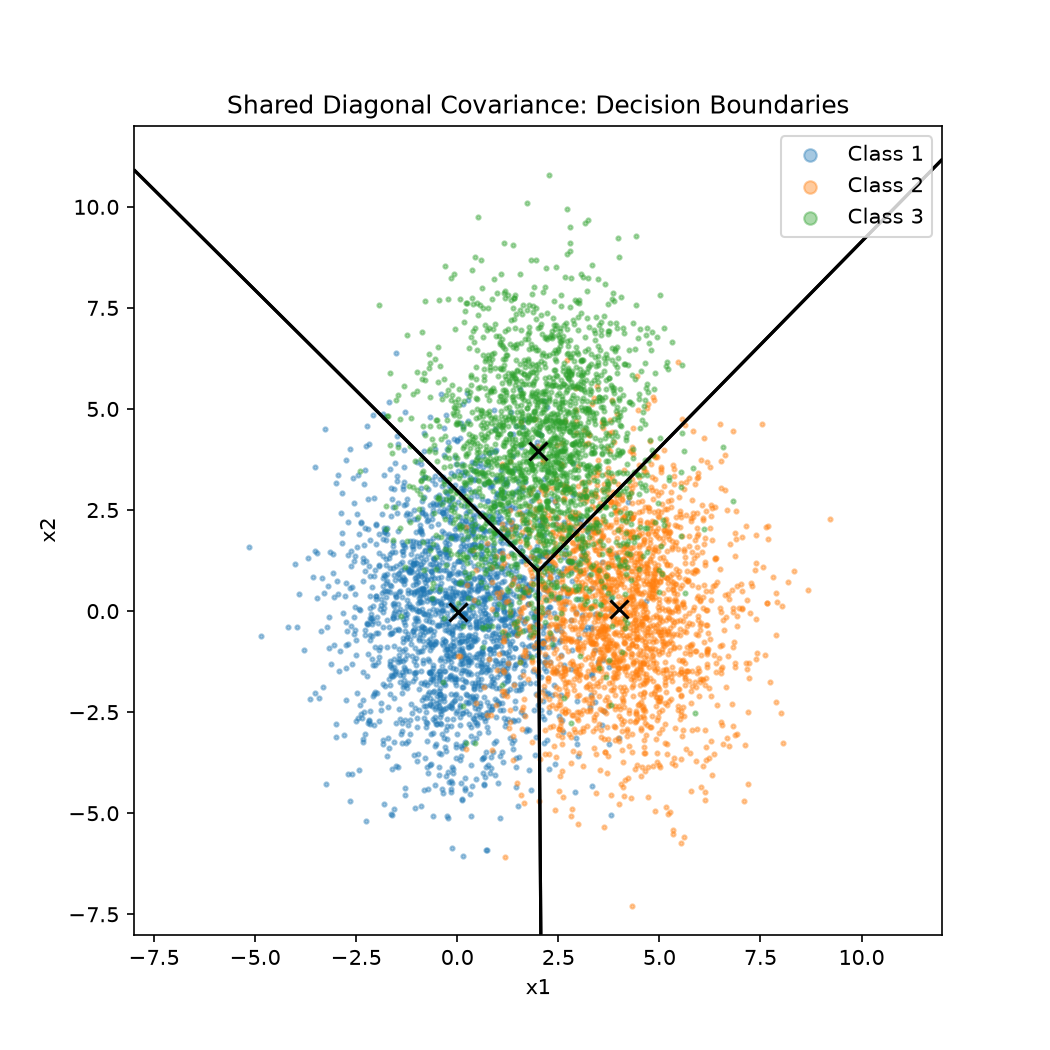
\includegraphics[width=\linewidth]{shared_diagonal_boundary.png}
\caption{Shared covariance}
\end{subfigure}
\hfill
\begin{subfigure}[t]{0.48\textwidth}
\centering
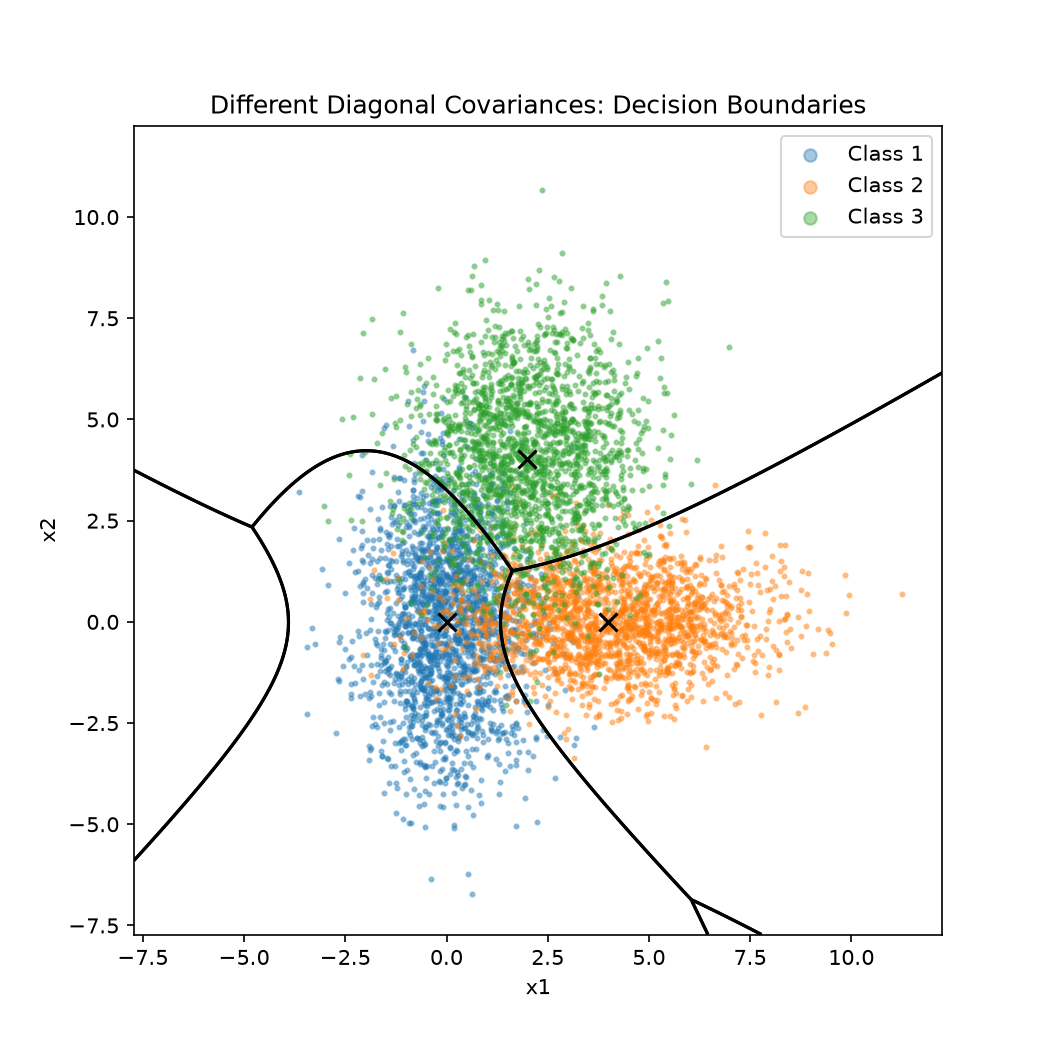
\includegraphics[width=\linewidth]{different_diagonal_boundary.png}
\caption{Different covariance}
\end{subfigure}
\caption{Test points and decision boundaries for diagonal covariance.}
\end{figure}
\vspace{7mm}
\begin{minipage}[t]{0.48\textwidth}
\small
\textbf{Shared: 82.73\% accuracy}\\[3pt]
\textbf{Estimated means}\\[-2pt]
\begin{tabular}{ccc}
\toprule
Class & $\hat\mu_1$ & $\hat\mu_2$ \\
\midrule
1 & 0.01 & -0.01 \\
2 & 4.01 & 0.05 \\
3 & 2.00 & 3.97 \\
\bottomrule
\end{tabular}\\[5pt]
\textbf{Covariance: generating / estimated}\\[-2pt]
\begin{tabular}{cll}
\toprule
Class & Generating & Estimated \\
\midrule
1 & (2.00, 4.00) & (2.00, 3.97) \\
2 & (2.00, 4.00) & (2.00, 3.97) \\
3 & (2.00, 4.00) & (2.00, 3.97) \\
\bottomrule
\end{tabular}\\[5pt]
\textbf{Confusion matrix} (rows: true; columns: predicted)\\[-2pt]
\begin{tabular}{c|ccc}
 & 1 & 2 & 3 \\
\hline
1 & 1671 & 135 & 194 \\
2 & 109 & 1712 & 179 \\
3 & 218 & 201 & 1581 \\
\end{tabular}
\end{minipage}
\hfill
\begin{minipage}[t]{0.48\textwidth}
\small
\textbf{Different: 87.37\% accuracy}\\[3pt]
\textbf{Estimated means}\\[-2pt]
\begin{tabular}{ccc}
\toprule
Class & $\hat\mu_1$ & $\hat\mu_2$ \\
\midrule
1 & 0.02 & 0.01 \\
2 & 3.99 & -0.01 \\
3 & 2.00 & 4.02 \\
\bottomrule
\end{tabular}\\[5pt]
\textbf{Covariance: generating / estimated}\\[-2pt]
\begin{tabular}{cll}
\toprule
Class & Generating & Estimated \\
\midrule
1 & (1.00, 4.00) & (1.00, 4.09) \\
2 & (4.00, 1.00) & (4.07, 1.01) \\
3 & (2.00, 3.00) & (2.00, 3.03) \\
\bottomrule
\end{tabular}\\[5pt]
\textbf{Confusion matrix} (rows: true; columns: predicted)\\[-2pt]
\begin{tabular}{c|ccc}
 & 1 & 2 & 3 \\
\hline
1 & 1762 & 106 & 132 \\
2 & 192 & 1746 & 62 \\
3 & 161 & 105 & 1734 \\
\end{tabular}
\end{minipage}
% Add observations in the student's own words.
\newpage
\section*{Full covariance}
\textit{Covariance entries below show $(\Sigma_{11},\Sigma_{12},\Sigma_{22})$.}
\begin{figure}[H]
\centering
\begin{subfigure}[t]{0.48\textwidth}
\centering
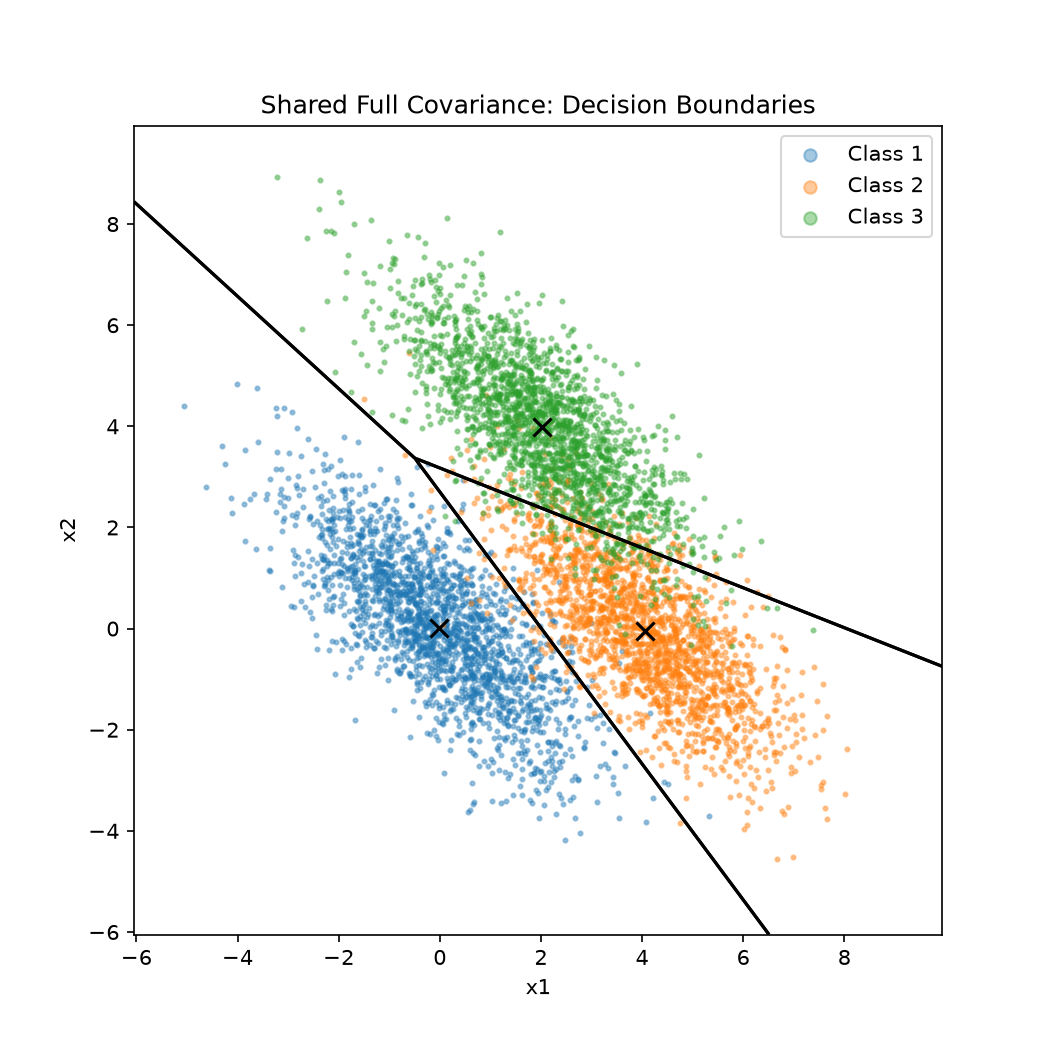
\includegraphics[width=\linewidth]{shared_full_boundary.png}
\caption{Shared covariance}
\end{subfigure}
\hfill
\begin{subfigure}[t]{0.48\textwidth}
\centering
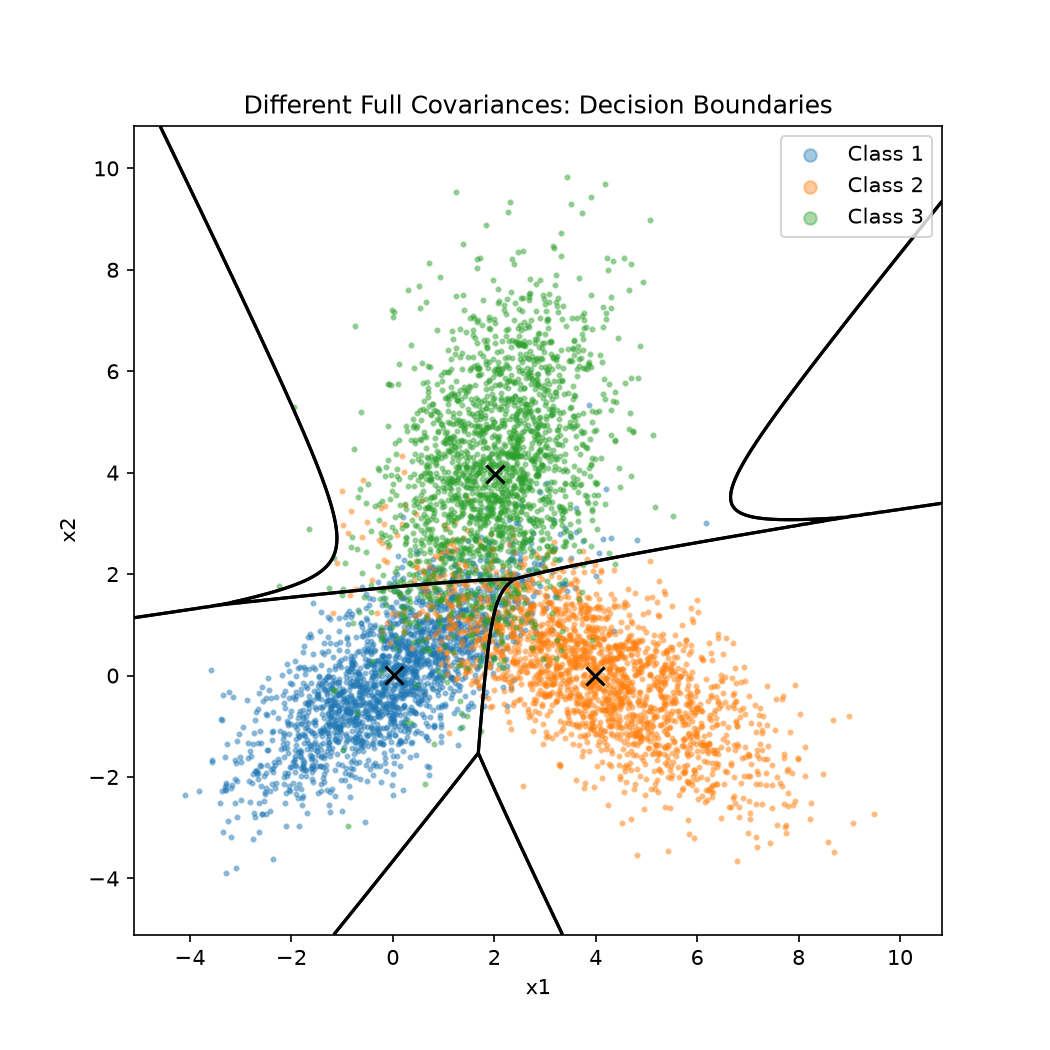
\includegraphics[width=\linewidth]{different_full_boundary.png}
\caption{Different covariance}
\end{subfigure}
\caption{Test points and decision boundaries for full covariance.}
\end{figure}
\vspace{7mm}
\begin{minipage}[t]{0.48\textwidth}
\small
\textbf{Shared: 94.45\% accuracy}\\[3pt]
\textbf{Estimated means}\\[-2pt]
\begin{tabular}{ccc}
\toprule
Class & $\hat\mu_1$ & $\hat\mu_2$ \\
\midrule
1 & -0.01 & 0.01 \\
2 & 4.06 & -0.04 \\
3 & 2.03 & 3.99 \\
\bottomrule
\end{tabular}\\[5pt]
\textbf{Covariance: generating / estimated}\\[-2pt]
\begin{tabular}{cll}
\toprule
Class & Generating & Estimated \\
\midrule
1 & (2.00, -1.50, 2.00) & (2.00, -1.50, 2.01) \\
2 & (2.00, -1.50, 2.00) & (2.00, -1.50, 2.01) \\
3 & (2.00, -1.50, 2.00) & (2.00, -1.50, 2.01) \\
\bottomrule
\end{tabular}\\[5pt]
\textbf{Confusion matrix} (rows: true; columns: predicted)\\[-2pt]
\begin{tabular}{c|ccc}
 & 1 & 2 & 3 \\
\hline
1 & 1962 & 38 & 0 \\
2 & 40 & 1828 & 132 \\
3 & 2 & 121 & 1877 \\
\end{tabular}
\end{minipage}
\hfill
\begin{minipage}[t]{0.48\textwidth}
\small
\textbf{Different: 87.53\% accuracy}\\[3pt]
\textbf{Estimated means}\\[-2pt]
\begin{tabular}{ccc}
\toprule
Class & $\hat\mu_1$ & $\hat\mu_2$ \\
\midrule
1 & 0.02 & 0.00 \\
2 & 4.00 & -0.00 \\
3 & 2.02 & 3.98 \\
\bottomrule
\end{tabular}\\[5pt]
\textbf{Covariance: generating / estimated}\\[-2pt]
\begin{tabular}{cll}
\toprule
Class & Generating & Estimated \\
\midrule
1 & (2.00, 1.30, 1.50) & (2.00, 1.29, 1.48) \\
2 & (3.00, -1.50, 1.50) & (3.00, -1.51, 1.51) \\
3 & (1.20, 0.70, 3.00) & (1.17, 0.66, 2.95) \\
\bottomrule
\end{tabular}\\[5pt]
\textbf{Confusion matrix} (rows: true; columns: predicted)\\[-2pt]
\begin{tabular}{c|ccc}
 & 1 & 2 & 3 \\
\hline
1 & 1756 & 108 & 136 \\
2 & 175 & 1709 & 116 \\
3 & 153 & 60 & 1787 \\
\end{tabular}
\end{minipage}
% Add observations in the student's own words.
\end{document}
